\documentclass[12pt]{article}
\usepackage{amsmath, graphicx, caption,array, amsthm}
\usepackage{amsfonts, xcolor, physics, listings,verbatim}
\usepackage{amssymb,empheq, mathrsfs, comment, subfig, hyperref, url, fancyhdr, tikz, booktabs, geometry, enumitem, textcomp, subfig}
\usepackage[T1]{fontenc} % for \symbol{92} 
% Command "alignedbox{}{}" for a box within an align environment
% Source: http://www.latex-community.org/forum/viewtopic.php?f=46&t=8144
\newlength\dlf  % Define a new measure, dlf
\newcommand\alignedbox[2]{
% Argument #1 = before & if there were no box (lhs)
% Argument #2 = after & if there were no box (rhs)
&  % Alignment sign of the line
{
\settowidth\dlf{$\displaystyle #1$}  
    % The width of \dlf is the width of the lhs, with a displaystyle font
\addtolength\dlf{\fboxsep+\fboxrule}  
    % Add to it the distance to the box, and the width of the line of the box
\hspace{-\dlf}  
    % Move everything dlf units to the left, so that & #1 #2 is aligned under #1 & #2
\boxed{#1 #2}
    % Put a box around lhs and rhs
}
}

\addtolength{\oddsidemargin}{-1in}
\addtolength{\evensidemargin}{-1in}
\addtolength{\textwidth}{1.75in}
\addtolength{\topmargin}{-1in}
\addtolength{\textheight}{1.75in}
\newcommand{\contra}{$\rightarrow\leftarrow$}
\newcommand{\tb}{  \textbackslash  }
\newcommand{\bj}{\ \Longleftrightarrow \ }

%bailey meche
\begin{document}
%bailey meche
	\begin{center}
		ECMA 33230: Macroeconomic Crises - Spring 2025\\
        Problem Set 3: Bank Runs \\
		Due Date: May 18, 2025 \\
        Bailey Meche
	\end{center}

\subsection*{1. (5 points) Banks as liquidity providers:}

\begin{enumerate}[label=(\alph*)]
    \item (2 points) Define ``liquidity'' in words.
    \subsubsection*{Solution}

    Liquidity measures how easily, quickly, and cheaply you can convert an asset into cash. 

    \item (3 points) Decide for each of the following assets if it’s relatively liquid or relatively illiquid: a factory plant, stocks, bonds, balance in your checking account, a piece of land, real estate, a gold ring, Bitcoin.
     \subsubsection*{Solution}

     A factory plant, bonds,  a piece of land, real estate, and a gold ring are relatively illiquid. Each of these involve significant search frictions and other market frictions to convert into cash.  Stocks, bonds, balance in your checking account, and Bitcoin are relatively liquid. 
     
%\subsubsection*{\textcolor{red}{todo}}
     
\end{enumerate}

\subsection*{2. (15 points)}

An asset that is purchased in period 0 pays out a return $R_1$ in period 1 or a return $R_2$ in period 2. Assume $R_2 \geq R_1$ and that $R_2$ is only earned if the asset is not liquidated in period 1. Imagine a consumer has preferences $(1 - \theta)u(c_1) + \theta u(c_2)$, where $\theta \in \{0, 1\}$ 
is a bivariate iid random variable with $\Pr(\theta = 0) = \pi = 0.25$. A consumer invests $x = 2$ in period 0 but has the choice between two assets. Asset A gives returns $R_{1}^A = 1$, $R_{2}^A = 2$ and asset B earns the returns $R_{1}^B = 1.25$, $R_{2}^B = 1.85$.

\begin{enumerate}[label=(\alph*)]
    \item (3 points) Derive formally the household’s expected utility function $EU$ in terms of $\pi$, $c_1$ and $c_2$, starting from the preferences given in the question. Show all steps of your derivation.

    \subsubsection*{Solution}
    \begin{align*}
    U &= (1 - \theta)u(c_1) + \theta u(c_2)
    \\ EU = \mathbb{E}[U]&= \mathbb{E}\left((1 - \theta)u(c_1) + \theta u(c_2)\right)
    \\      &= \pi u(c_1) + (1-\pi) u(c_2)
    \end{align*}

    \item (2 points) What is the degree of liquidity of an asset in terms of $R_1$ and $R_2$? What is the degree of liquidity of cash? Is cash liquid or illiquid?
    \subsubsection*{Solution}

    \begin{align*}
        \text{degree of liquidity for A} &= \frac{R_1}{R_2} = \frac{1}{2} = 0.5
        \\ \text{degree of liquidity for B} &= \frac{R_1}{R_2} = \frac{1.25}{1.85} = 0.676
    \end{align*}
    Degree of liquidity of cash is 1. Cash is the baseline for liquidity as it is the standard liquid asset when considering US assets. 
    

    \item (1 point) Is asset A or asset B more liquid?
    \subsubsection*{Solution}

    From (b), we can see that asset $B$ is more liquid since $\frac{R_1^A}{R_2^A} < \frac{R_1^B}{R_2^B}$ where liquidity increases as $l\to 1.$

    \item (2 points) What are the maximum consumption levels $c_1$ and $c_2$ if the entire investment is used to purchase asset A in period 0? What are $c_1$ and $c_2$ if asset B is purchased instead?
    \subsubsection*{Solution}

    If the entire investment $x=2$ is used to purchase asset A in period 0, the  maximum consumption levels are:
    \begin{equation}\label{2d_1}
        \begin{cases}
        c_1 = R_{1}^Ax = 2 & t=1
        \\ c_2 = R_{2}^Ax = 4 & t=2
    \end{cases}
    \end{equation}
    If the entire investment $x=2$ is used to purchase asset B in period 0, the  maximum consumption levels are:
    \begin{equation}\label{2d_2}
        \begin{cases}
        c_1 = R_{1}^Bx = 2.5 & t=1
        \\ c_2 = R_{2}^Ax = 3.7 & t=2
    \end{cases}
    \end{equation}


    \item (2 points) For $u(c) = 1 - \frac{1}{c}$, what is the expected utility for the consumer if the entire investment is used to purchase asset A? 
    What is the expected utility if the consumer invests everything in asset B instead? In which asset will the consumer optimally invest?
    \subsubsection*{Solution}

    If the entire investment $x=2$ is used to purchase asset A in period 0, then the expected utility is
    \begin{align*}
        EU_A &=  \pi u(c_1) + (1-\pi) u(c_2)
        \\ &= 0.25 \cdot u(2) + 0.75 \cdot u(4) & \text{From \eqref{2d_1}}
        \\ &= 0.25 \cdot  \left(1 - \frac{1}{2}\right) + 0.75 \cdot \left(1 - \frac{1}{4}\right)
        \\ &= \frac{11}{16} = 0.6875
    \end{align*}
    If the entire investment $x=2$ is used to purchase asset B in period 0, then the expected utility  is
    \begin{align*}
        EU_B &=  \pi u(c_1) + (1-\pi) u(c_2)
        \\ &= 0.25 \cdot u(2.5) + 0.75 \cdot u(3.7) & \text{From \eqref{2d_2}}
        \\ &= 0.25 \cdot  \left(1 - \frac{1}{2.5}\right) + 0.75 \cdot \left(1 - \frac{1}{3.7}\right)
        \\ &= \frac{129}{185} \approx 0.697
    \end{align*}
    Given that $EU_B > EU_A$,  the risk-averse consumer will optimally invest in asset B.


    \item (5 points) Repeat part (e) for $u(c) = c - 2.5$. If you compare your results to part (e), why does this reflect that risk aversion creates demand for liquidity? Provide intuition.
    \subsubsection*{Solution}

     If the entire investment $x=2$ is used to purchase asset A in period 0, then the expected utility is
    \begin{align*}
        EU_A &=  \pi u(c_1) + (1-\pi) u(c_2)
        \\ &= 0.25 \cdot u(2) + 0.75 \cdot u(4) & \text{From \eqref{2d_1}}
        \\ &= 0.25 \cdot  \left(2 - 2.5\right) + 0.75 \cdot \left(4-2.5\right)
        \\ &= 1
    \end{align*}
    If the entire investment $x=2$ is used to purchase asset B in period 0, then the expected utility  is
    \begin{align*}
        EU_B &=  \pi u(c_1) + (1-\pi) u(c_2)
        \\ &= 0.25 \cdot u(2.5) + 0.75 \cdot u(3.7) & \text{From \eqref{2d_2}}
        \\ &= 0.25 \cdot  \left(2.5-2.5\right) + 0.75 \cdot \left(3.7-2.5\right)
        \\ &= 0.9
    \end{align*}
    Given that $EU_A > EU_B$,  the risk-neutral consumer will optimally invest in asset $A$.
    \end{enumerate}

\subsection*{3. (25 points)}

Consumers live for three periods, $t = 0, 1, 2$. In period 0, each consumer has an endowment of $B = 1.5$ and decides which part of the endowment to store $y$ or invest $x$. Investment earns a return $R = 1.3$ in period 2 and has a liquidation return of $L = 0.8$ in period 1. Consumers have utility $(1-\theta)u(c_1)+\theta u(c_2)$ where $u(c) = \frac{c^{1-\sigma}}{1-\sigma}$, with $\sigma = 3$, and come in two types: impatient consumers ($\theta = 0$) only care about period 1 consumption $c_1$, and patient consumers ($\theta = 1$) only care about period 2 consumption $c_2$. Types are revealed in period 1 and $\pi = \Pr(\theta = 0) = 0.5$ with $\theta \in \{0, 1\}$ iid.

\begin{enumerate}[label=(\alph*)]
    \item (4 points) Calculate the equilibrium levels for investment $x$, consumption $c_1$ and $c_2$ and the corresponding expected utility under autarky. How would these values change if liquidation was entirely ruled out?
    \subsubsection*{Solution}

    For consumer utility $(1-\theta)u(c_1)+\theta u(c_2)$ where $u(c) = \frac{c^{1-\sigma}}{1-\sigma}$, we have the household's problem in the autarky: 
    \begin{align*}
        &\max_{c_1, c_2, x,y} \pi u(c_1) + (1-\pi)u(c_2) && s.t. && \begin{cases}
            B  =x+y & t=0
            \\ c_1 \leq y + Lx = B-x+Lx & t=1
            \\ c_2 \leq y + Rx = B-x + Rx & t=2
        \end{cases}
        \\ &\max_{c_1, c_2, x,y} \frac{1}{2} \cdot  \frac{c_1^{1-\sigma}}{1-\sigma} + \frac{1}{2} \cdot  \frac{c_2^{1-\sigma}}{1-\sigma}&& s.t. && \begin{cases}
            1.5  =x+y & t=0
            \\ c_1 \leq 1.5-x(1-L) & t=1
            \\ c_2 \leq 1.5+x(R-1) & t=2
        \end{cases}
        \\ &-\frac{1}{4}\max_{c_1, c_2, x,y} \frac{1}{c_{1}^{2}}+\frac{1}{c_{2}^{2}}  && s.t. && \begin{cases}
             1.5 =x+y & t=0
            \\ c_1 \leq 1.5-0.2x  & t=1
            \\ c_2 \leq 1.5+0.3x & t=2
        \end{cases}
    \end{align*}
    Taking FOCs, we know that 
    \begin{align*}
         \frac{u'(c_1)}{u'(c_2)} &= \frac{(1-\pi)(R-1)}{\pi(1-L)} 
         \\  \frac{c_1^{-2}} {c_2^{-2}}&= 1.5
         \\ \frac{c_1}{c_2}&= \frac{1}{\sqrt{1.5}}\approx 0.816
         \\ c_2 &= c_1 \sqrt{1.5}
    \end{align*}
    This result lies in the interior solution $x\in(0,1)$, so using this to solve for $x$:
    \begin{align*}
       1.5+0.3x = c_2 &= \sqrt{1.5}c_1  = \sqrt{1.5}(1.5-0.2x)
       \\  1.5\left(1-\sqrt{1.5}\right)&=\left(-0.3-0.2\sqrt{1.5}\right)x
       \\ x\ &= -30+25\sqrt{1.5} \approx 0.6186
       \\ c_1 &= 1.5-0.2\cdot 5(-6+5\sqrt{1.5}) = 7.5-5\sqrt{1.5} \approx 1.376
       \\ c_2 &= 1.5+0.3\cdot 5(-6+5\sqrt{1.5}) = 7.5\left(-1+\sqrt{1.5}\right) \approx 1.686
    \end{align*}
    which checks out since $c_1<c_2.$
    The expected utility in this case is given by 
    \[ EU = -\frac{1}{4}\left( \frac{1}{(7.5-5\sqrt{1.5})^{2}}+\frac{1}{\left(7.5\left(-1+\sqrt{1.5}\right)\right) ^{2}} \right) \approx -0.220.\]
    
    \bigskip 
    If liquidation was ruled out, then impatient consumers $(\theta=0)$ cannot recover any invested funds at $t=1$, so $L=0$. Such consumers can still choose to store or invest.
    \begin{align*}
        &-\frac{1}{4}\max_{c_1, c_2, x,y} \frac{1}{c_{1}^{2}}+\frac{1}{c_{2}^{2}}  && s.t. && \begin{cases}
             1.5 =x+y & t=0
            \\ c_1 \leq 1.5-x  & t=1
            \\ c_2 \leq 1.5+0.3x & t=2
        \end{cases}
    \end{align*}
    Taking FOCs, we know that 
    \begin{align*}
         \frac{u'(c_1)}{u'(c_2)} &= \frac{(1-\pi)(R-1)}{\pi} 
         \\  \frac{c_1^{-2}} {c_2^{-2}}&= 0.3
         \\ \frac{c_1}{c_2}&= \frac{1}{\sqrt{0.3}}\approx 1.826
         \\ c_2 &= c_1 \sqrt{0.3}
    \end{align*}
    Solving for $x$:
    \begin{align*}
       1.5+0.3x = c_2 &= \sqrt{0.3}c_1  = \sqrt{0.3}( 1.5-x)
       \\ x\ &= \frac{1.5\left(1-\sqrt{0.3}\right)}{-0.3-\sqrt{0.3}} \approx -0.8<0
       %\\ c_1 &= 1.5-0.2\cdot 5(-6+5\sqrt{1.5}) = 7.5-5\sqrt{1.5} \approx 1.376
      % \\ c_2 &= 1.5+0.3\cdot 5(-6+5\sqrt{1.5}) = 7.5\left(-1+\sqrt{1.5}\right) \approx 1.686
    \end{align*}
    which is infeasible since $x \in [0,1]$. Hence, the optimal investment is $x=0$ wherein 
    \[ c_1 =  c_2 = 1.5.\]
    The expected utility in this case is given by 
    \[ EU = -\frac{1}{4}\left( \frac{1}{(1.5)^{2}}+\frac{1}{(1.5)^{2}} \right) = -\frac{2}{9}\approx -0.222. \]
    
    \item (2 points) Set up a consumer’s incomplete market problem in period 0 with the possibility to trade in period 1. What are the market equilibrium consumption levels $c_1$ and $c_2$ and the associated expected utility level?
\subsubsection*{Solution}

    For a market setup in $t=0$, early consumers have the possibility to trade at price $P$ in $t=1$ with the possibility of return $R$ in $t=2$.
    For consumer utility $(1-\theta)u(c_1)+\theta u(c_2)$ where $u(c) = \frac{c^{1-\sigma}}{1-\sigma}$, we have the household's problem in the market: 
    \begin{align*}
        &\max_{c_1, c_2, x,y} \pi u(c_1) + (1-\pi)u(c_2) && s.t. && \begin{cases}
            B  =x+y & t=0
            \\ c_1 \leq y + Px & t=1
            \\ c_2 \leq \left(x + \frac{y}{P}\right)R & t=2
        \end{cases}
        \\ &-\frac{1}{4}\max_{c_1, c_2, x,y} \frac{1}{c_{1}^{2}}+\frac{1}{c_{2}^{2}}  && s.t. && \begin{cases}
             1.5 =x+y & t=0
            \\ c_1 \leq 1.5 + (P-1)x & t=1
            \\ c_2 \leq R\left(x + \frac{1.5-x}{P}\right) & t=2
        \end{cases}
    \end{align*}
    With competitive agents, we have the market of the illiquid asset $P=1.$ This gives consumption
    \begin{align*}
         c_1 &= 1.5;  &c_2 &= 1.5R
    \end{align*}
    and expected utility 
    \[ EU = -\frac{1}{4}\left( \frac{1}{(1.5)^{2}}+\frac{1}{(1.5(1.3))^{2}} \right) = -\frac{269}{1521} \approx -0.1777. \]


    \item (2 points) Compute the equilibrium levels for investment $x$, consumption $c_1$ and $c_2$ and the corresponding expected utility in an economy with financial intermediation. Assume the banking system achieves the good Nash equilibrium.
\subsubsection*{Solution}

    For consumer utility $(1-\theta)u(c_1)+\theta u(c_2)$ where $u(c) = \frac{c^{1-\sigma}}{1-\sigma}$, we have the household's problem in an economy with financial intermediation: 
    \begin{align*}
        &\max_{c_1, c_2, x,y} \pi u(c_1) + (1-\pi)u(c_2) && s.t. && \begin{cases}
            B  =x+y & t=0
            \\ \pi c_1 =y & t=1
            \\ (1-\pi) c_2 = Rx & t=2
        \end{cases}
    \end{align*}
    Taking FOCs, we know that 
    \begin{align*}
         \frac{u'(c_1)}{u'(c_2)} &= R
         \\ \frac{u'\left(\frac{1.5-x}{\pi}\right)}{u'\left(\frac{Rx}{1-\pi}\right)} &=
         \\ \frac{\left(\frac{1.5-x}{\pi}\right)^{-2}}{\left(\frac{Rx}{1-\pi}\right)^{-2}}&=1.3
         \\ \frac{1.5-x}{\pi}\left(\frac{1-\pi}{Rx}\right) &= \frac{1}{\sqrt{1.3}}
    \end{align*}
    which provides 
    \begin{empheq}[box=\fbox]{align*}
           x&= 5\sqrt{1.3}-5 \approx 0.7
       \\   c_1 &= \frac{1.5-x}{\pi} \approx 1.598
       \\ c_2 &= \frac{Rx}{1-\pi} \approx 1.82 > c_1 
       \\  EU &= -\frac{1}{4}\left( \frac{1}{\left(\frac{1.5-x}{\pi}\right)^{2}}+\frac{1}{\left(\frac{Rx}{1-\pi}\right)^{2}} \right) \approx -0.173
    \end{empheq}
    assuming that banks choose the good Nash equilibrium.



    \item (8 points) Plot the feasible sets under autarky and under financial intermediation in a $(c_1, c_2)$-graph. Then add the indifference curves that are associated with your results from parts (a), (b) and (c) in the plot. Use Julia to make this plot and include your code.
\subsubsection*{Solution}

    See Figure \eqref{fig:4} for this plot.
    \begin{figure}[h]
            \centering
                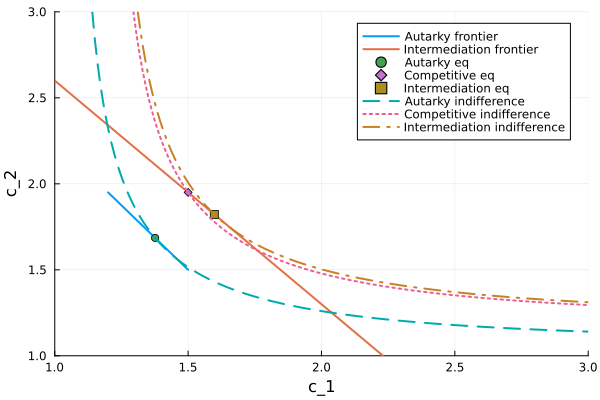
\includegraphics[width=0.65\textwidth]{feasible_sets_and_indiff.png}
                \caption{Problem 3: feasible sets and indifference curves}
                \label{fig:4}
        \end{figure}

    \item (2 points) Why can maturity mismatch in bank’s balance sheet lead to a worse outcome than in part (c)? Provide intuition.
\subsubsection*{Solution}

% \subsubsection*{\textcolor{red}{todo}}
%pg. 8
A maturity mismatch in a bank’s balance sheet is characterized by short-term assets $y$ and long-term assets $x$ with deposits $B$ for short-term liabilities.  
This maturity mismatch lies in the fact that if $c_1^B > y$, the bank will not be liquid enough to provide the demanded withdraw amount since $x$ is inaccessible in $t=1.$ Since this overdrawing effect can only happen as a result of actions by late consumers, this is known as a coordination failure among late consumers. 

In financial intermediation economy from part (c), banks are able to fully observe $\pi$ and provide an incentive-compatible allocation with incomplete insurance $(c_1^B< c_2^B)$ and protect against late-type consumers withdrawing in $t=1.$
When late-type consumers  withdraw in $t=1$, everyone is worse off. 
If a  late-type consumer $i$ perceives that all other late types  $-i$ in $t=1$ are running, they themselves will run and receive a payoff of $y+Lx$ instead of 0. In this case, all late-type consumers receive $y+Lx$ isnsntead of the full $c_2^B > 1> y+Lx $.

    \item (3 points) Suppose the government wants to insure deposits by imposing a tax on early withdrawals to rule out bank runs. Explain how the government could do this. What is the tax rate the government sets to achieve the first best?
\subsubsection*{Solution}
    % The government insures banks' deposits to prevent runs by taxing consumers in $t=1$ based on realized $f$ (fraction of consumers trying to withdraw, giving the proceeds back to banks) wherein we have the first-best pre-tax consumption  $c_1^*, c_2^*$ and tax rate that achieves the first best consumption levels 
    % \[ \tau = \begin{cases}
    %     0 & f \leq \pi 
    %     \\ 1 - \frac{1}{c_1} & f > \pi 
    % \end{cases}.\]

    % Setting up this problem to achieve first best levels, 
    % \begin{align*}
    %     &\max_{c_1, c_2, x,y} \pi u(c_1) + (1-\pi)u(c_2) && s.t. && \begin{cases}
    %         B  =x+y & t=0
    %         \\ \pi c_1 =y & t=1
    %         \\ (1-\pi) c_2 = Rx & t=2
    %     \end{cases}
    % \end{align*}

    In this case, the government insures banks' deposits to prevent runs by taxing consumers in $t=1$ based on realized $f$ (fraction of consumers trying to withdraw, giving the proceeds back to banks) compared to the known $\pi$.
    The rule  for such a tax would be 
    \[ \tau = \begin{cases}
        0 & f \leq \pi 
        \\ 1 - \frac{1}{c_1} & f > \pi 
    \end{cases}\]
    with the goal of $\tau$ using $c_1$ toward the first-best allocation $c_1^*$ wherein $f =\pi$. Recall that the financial intermediation case in part (c) achieves best-allocation, so we begin with this setup and introduce $\tau$. To use $\tau$ to discourage runs, we introduce tax from in $t=1$ where
    \begin{align*}
        &\max_{c_1, c_2, x,y} \pi u(c_1) + (1-\pi)u(c_2) && s.t. && \begin{cases}
            B  =x+y & t=0
            \\ \pi c_1 =y + \tau & t=1
            \\ (1-\pi) c_2 = Rx & t=2
        \end{cases}
    \end{align*}
    Now, the dominant strategy for late-type consumers is to wait (not run). The equilibrium consumption levels for this problem achieves the first best levels $c_1^*, c_2^*.$

    \item (4 points) Suppose there is deposit insurance in place. Calculate the consumption levels of a patient consumer who withdraws in period 1, in the two situations where more or less than the share of early consumers withdraw in period 1. Calculate the consumption levels of a patient consumer who withdraws in period 2, in the two situations where more or less than the share of early consumers withdraw in period 1.
    \subsubsection*{Solution}

    The consumptions for each type in each scenario for $f$ are given as: 

    
    %\begin{center}
        \begin{tabular}{|c|c|c|}
        \textbf{Early consumer $j$} & $t=1$ & $t=2$  \\
            \hline
            & \textbf{run} & \textbf{not run } \\
            \hline
            \textbf{ $f \leq \pi $} & $c_1^* = \frac{1.5-x}{\pi} \approx 1.598$ & $0$ \\
            \hline
            \textbf{$f > \pi $ } & $1 $ &  \\
            \hline
        \end{tabular}
    %\end{center}
     %\begin{center}
        \begin{tabular}{|c|c|c|}
        \textbf{Late consumer $j$}& $t=1$ & $t=2$\\
            \hline
            & \textbf{run} & \textbf{not run } \\
            \hline
            \textbf{$f \leq \pi $} & $c_1^* \approx 1.598$ & $c_2^*= \frac{Rx}{1-\pi} \approx 1.82$ \\
            \hline
            \textbf{$f > \pi $} & $1$ & $R=1.3$ \\
            \hline
        \end{tabular}
    %\end{center}

    
\end{enumerate}

\subsection*{4. (14 points)}

A measure 1 of consumers live for three periods, $t = 0, 1, 2$. In period 0 each consumer has an endowment of \$3 and decides which part of the endowment to store $y$ or invest $x$. Investment earns a return $R = 1.1$ in period 2. Consumers have expected utility function $EU = \pi u(c_1)+(1-\pi)u(c_2)$. In period 1 it is revealed if a consumer is an early type and only cares about consumption $c_1$ or a late type and only values $c_2$, where $\pi$ is the probability of being an early consumer. Early consumers can sell their investments to late consumers at price $P$ in period 1.

\begin{enumerate}[label=(\alph*)]
    \item (2 points) Write down the period-by-period budget constraints for a consumer.
    \subsubsection*{Solution}

    For a market setup, we have the consumer's problem 
    \begin{align*}
        &\max_{c_1, c_2, x,y} \pi u(c_1) + (1-\pi)u(c_2) && \text{with budget constraints:} && \begin{cases}
            3=B  =x+y & t=0
            \\ c_1 \leq y + Px & t=1
            \\ c_2 \leq \left(x + \frac{y}{P}\right)R & t=2
        \end{cases}
    \end{align*}

    \item (8 points) \textbf{Extra Credit:} Prove that $P = 1$ in equilibrium.
    \subsubsection*{Solution}

    %\subsubsection*{\textcolor{red}{todo}}
    Each ex‐ante identical consumer chooses $x\in[0,3]$ (invested at $t=0$) and $y=3-x$ (kept in “cash” for $t=1$) to maximize expected utility
    \begin{align*}
        &\max_{c_1, c_2, x,y} \pi u(c_1) + (1-\pi)u(c_2) && \text{with budget constraints:} && \begin{cases}
            3=B  =x+y & t=0
            \\ c_1 = y + P\,x = 3 - x + P\,x & t=1
            \\ c_2 = y + R\,x = 3 - x + R\,x & t=2
        \end{cases}
    \end{align*}
Taking FOCs:
\begin{equation}
    \pi\,(P-1)\,u'(c_1)\;+\;(1-\pi)\,(R-1)\,u'(c_2)\;=\;0.
\label{FOC}
\end{equation}
Because $R>1$ and $u'>0$, we have $(1-\pi)(R-1)u'(c_2)>0$.  Hence, we require
$$
P-1<0
\;\;\Longrightarrow\;\;
P<1.
$$
We know a necessary condition for an interior optimum is $P<1$.
Now note that any consumer who ends up being a late-type consumer could, at $t=1$,
either wait and get $c_2=3 - x + R\,x$ at $t=2$,
or buy additional units of the $t=2$ asset at price $P$ out of her $t=1$ resources $c_1 = 3 - x + P\,x$.

In a frictionless, competitive market those two must deliver the same  marginal payoff, or else you’d get infinite arbitrage.  In particular, buying one more unit at $t=1$ costs $P$ units of consumption then and yields $R$ units at $t=2$; the marginal rate at which $c_1$ trades off against $c_2$ is exactly the ratio of marginal utilities:
\begin{equation}
    \underbrace{P}_{\substack{\text{price at}~t=1}}
\;=\;
\underbrace{\frac{u'(c_2)}{u'(c_1)}}_{\substack{\text{marginal}\\\text{rate of substitution}}} \cdot R.
\label{No–arb}
\end{equation}
But from \eqref{FOC} we get
$$
\frac{u'(c_2)}{u'(c_1)}
\;=\;
\frac{\pi\,(1-P)}{(1-\pi)(R-1)}.
$$
Substitute  into the no-arbitrage condition:
$$
P
\;=\;
R 
\frac{\pi\,(1-P)}{(1-\pi)(R-1)}
\;\;\Longrightarrow\;\;
P\,\bigl[(1-\pi)(R-1) + \pi\,R \bigr]
\;=\;
\pi\,R.
$$
But $(1-\pi)(R-1) + \pi\,R = R - (1-\pi)$, so the bracket is strictly positive.  Solving for $P$ gives
$$
P \;=\;\frac{\pi\,R}{R - (1-\pi)}.
$$
On the other hand, plugging $P<1$ from the FOC into this formula forces the unique solution
$$
\boxed{P=1.}
$$

To verify, the FOC becomes $$\pi\cdot0 + (1-\pi)(R-1)u'(c_2)=0$$ which can only hold if $(1-\pi)(R-1)=0$.  Since $R>1$ and $\pi<1$, the only way is that the interior optimum disappears and we end up at a corner solution in which the marginal trades exactly offset.
The no-arbitrage condition reduces to $$1 = \dfrac{u'(c_2)}{u'(c_1)}R,$$ which requires $u'(c_1)=R\,u'(c_2)$.  Together with the resource constraint this pins down the unique competitive equilibrium consumption plan.

But since the only way both \eqref{FOC} and \eqref{No–arb} can be satisfied is by pushing the candidate interior solution into the corner and yielding consistency only at $P=1$, we conclude that the equilibrium price in the market outcome must be $P=1$.
    
    \item (2 points) How much do early and late types consume in the market equilibrium?
    \subsubsection*{Solution}

    In equilibrium where $P=1$, we have
    \[ c_1 =3, \quad c_2 = (3)(1.1) = 3.3\]

    
    \item (2 points) Assume $\pi = 0.1$, $u(c) = \frac{c^{1-\gamma}}{1- \gamma}$, $\gamma = 2$. What is the expected utility in the market?
    \subsubsection*{Solution}

    \begin{align*}
        EU &= \pi u(c_1) + (1-\pi)u(c_2) 
        \\ &= -0.1 c_1^{-1} - 0.9 c_2^{-1}
        \\ &= -0.1 (3)^{-1} - 0.9 (3.3)^{-1}
        \\ &= -\frac{101}{330} \approx -0.306
    \end{align*}


    
\end{enumerate}

\subsection*{5. (8 points) Bank Runs}

A demand deposit contract between bankers and consumers with endowment equal to 1 is $D = (c^B_1 = 1.04, c^B_2 = 1.06)$, where the subscripts refer to the period of withdrawal. The depositor Eva typically prefers to wait with a withdrawal until period 2, however she also knows that if a bank run occurs she can only withdraw 0.8 if she runs like everybody else or nothing if she is the only one who waits with the withdrawal to period 2.

\begin{enumerate}[label=(\alph*)]
    \item (4 points) Fill in the blank consumption level matrix to help Eva decide whether to run or not:
    \subsubsection*{Solution}

    Assuming that Eva is still able to make the choice for investment $x \in [0,1]$:    
    \begin{center}
        \begin{tabular}{|c|c|c|}
            \hline
            & \textbf{Everybody else Runs} & \textbf{Everybody else Does Not Run} \\
            \hline
            \textbf{Eva Runs} & $(\ 1-0.2x,\ 1-0.2x\ )$ & $(\ 1.04,\ 1.06\ )$ \\
            \hline
            \textbf{Eva Does Not Run} & $(\ 0 ,\ 1-0.2x\ )$ & $(\ 1.06 ,\ 1.06\ )$ \\
            \hline
        \end{tabular}
    \end{center}

    \item (2 points) How many (pure strategy) equilibria exist in this scenario? What are the associated payoffs?
    \subsubsection*{Solution}

    Two pure strategy equilibria exist here: 
    \begin{enumerate}
        \item (\textbf{Eva Does Not Run} , \textbf{Everybody else Does Not Run}) with payoff 1.06 for Eva. If everyone else doesn't run, 1.04 < 1.06.
        \item (\textbf{Eva Runs}, \textbf{Everybody else Runs}) with payoff $1-0.2x$ for Eva. If everyone else runs, $1-0.2x > 0.$
    \end{enumerate}

    \item (2 points) Under what conditions do all consumers withdraw in period $t = 1$ in a good Nash equilibrium?
    \subsubsection*{Solution}

    %\subsubsection*{\textcolor{red}{todo}}
    For all consumers to optimally withdraw in period $t = 1$ while still in a good Nash equilibrium, it must be that $c_1 \geq c_2.$
    
\end{enumerate}

\subsection*{6. (5 points)}

Why is the stockpiling and rationing of toilet paper at the beginning of the Corona Crisis sometimes referred to as a “run”? Explain the similarities to a bank run.
\subsubsection*{Solution}

%\subsubsection*{\textcolor{red}{todo}}
The toilet paper run of 2020 is similar to a bank run in several ways. 
In bank runs, if any one household believes others will withdraw, the agent will rush to the bank so they aren’t left holding worthless deposit claims.
Similarly in the toilet paper run, if you think others will stock up, you buy extra rolls even if you don’t need them; otherwise, there won’t be any left.
Both crises are driven not by an underlying fundamental scarcity (most banks were solvent/stores had supply chains intact), but by a coordination failure. Once enough people believe a shortage is coming and start withdrawing/buying, they create the very shortage they feared.
Banks normally hold only a small fraction of deposits in cash, trusting that not everyone will withdraw at once. Stores likewise keep limited stock on shelves, replenishing from warehouses “just in time.” In both cases, a simultaneous surge in demand overwhelms those buffers.
There are “good” and “bad”  (panic run / hoard) equilibria. Absent a coordinating mechanism (deposit insurance, purchase limits), rational agents gravitate to the bad equilibrium out of precaution.






\end{document}